\documentclass{sig-alternate-05-2015}
\usepackage{graphicx}
\graphicspath{ {images/} }
\usepackage{amsmath}

\begin{document}
\title{An Empirical Evaluation of BugLocatorII}

\numberofauthors{1}

\author{
\alignauthor
Juan Manuel Florez Fandino, Raul Quinonez Tirado \\ 
       \affaddr{University of Texas at Dallas}\\
       \affaddr{800 W. Campbell Road}\\
       \affaddr{Richardson, TX}\\
       \email{\{jflorez, Rxq100020\}@utdallas.edu}
}

\maketitle
\begin{abstract}

Faults or bugs are an inevitable part of software development. Bug reports are normally used to let developers know 
there is an error in the code, but they rarely provide all the information necessary to determine where the bug must be 
fixed at first glance. There is also no standardization or formal method of submitting bug reports. This hinders the performance of programmers, who will potentially have to revise large sections of code in order to locate the fault. This paper proposes a reimplementation of a tool for bug-report-based fault localization and an empirical study to assess its performance on a set of bug reports collected manually. We conclude with a comparison of this method with a baseline approach using standard Information Retrieval techniques.
\end{abstract}

%
% The code below should be generated by the tool at
% http://dl.acm.org/ccs.cfm
% Please copy and paste the code instead of the example below. 
%

%\begin{CCSXML}
%<ccs2012>
%<concept>
%<concept_id>10010583.10010717.10010733.10010734</concept_id>
%<concept_desc>Hardware~Bug detection, localization and diagnosis</concept_desc>
%<concept_significance>500</concept_significance>
%</concept>
%<concept>
%<concept_id>10002951.10003317.10003347.10003349</concept_id>
%<concept_desc>Information systems~Document filtering</concept_desc>
%<concept_significance>300</concept_significance>
%</concept>
%<concept>
%<concept_id>10002951.10003317.10003359.10003362</concept_id>
%<concept_desc>Information systems~Retrieval effectiveness</concept_desc>
%<concept_significance>300</concept_significance>
%</concept>
%<concept>
%<concept_id>10011007.10011074.10011099</concept_id>
%<concept_desc>Software and its engineering~Software verification and validation</concept_desc>
%<concept_significance>300</concept_significance>
%</concept>
%</ccs2012>
%\end{CCSXML}
%
%\ccsdesc[500]{Hardware~Bug detection, localization and diagnosis}
%\ccsdesc[300]{Information systems~Document filtering}
%\ccsdesc[300]{Information systems~Retrieval effectiveness}
%\ccsdesc[300]{Software and its engineering~Software verification and validation}


%
% End generated code
%

%
%  Use this command to print the description
%
\printccsdesc

\keywords{Bug localization; information retrieval; text processing; vector space model}

\section{Introduction}
Due to the inherent complexity of software products, the occurrence of bugs is inevitable. Many different methods
are used to prevent and repair faults in source code. However, on occasion these faults are not identified during
testing, instead being uncovered by the final users. Bug reports are used by both open source communities and
software development companies, and they allow users to communicate software failures to the development team.
These reports are usually submitted by making use of a bug-tracking system.
Once a bug report is received the usual process starts by assessing the severity of the bug and then assigning a
developer or group of developers the task of locating and fixing the bug.

However, locating bugs is usually not a straightforward process. Software systems that have the need of using
bug-tracking systems are usually too complex for any one person to be able to identify the possible location
of a bug at first
glance. Manually searching through the source code files would be prohibitively time-consuming in addition to
being error-prone. This is why many approaches for automated bug localization have been proposed. % REF?

Some of these approaches exploit the fact that source code is essentially text to allow search over code bases the
same way search over natural-language texts would be carried out. Information retrieval (IR) is the discipline
that studies search over corpora of unstructured data, and these approaches apply techniques born in this
field of study to bug localization.
One of the ways of locating software faults using IR is using a textual bug report and 
a collection of source code files \cite{le2014}. The system then will output a ranked list of files where
the bug is likely to be located. Developers will then look at the highest ranked locations for the bug first. 
Our goal for this project is to test a particular approach on a set of bug reports collected by our team.

The source code and data for this project are hosted on GitHub\footnote{https://github.com/jmflorezff/testing-project}.

\section{Problem}
Reimplementing a bug-report-based bug localization technique and testing it empirically on data collected by our team. We call
out implementation \emph{BugLocatorII}. The implementation will later be tested with data collected from open-source Java projects.

\section{Background}

\subsection{IR-Based Bug Localization}
Information Retrieval (IR) can be defined as the process of finding material of an unstructured nature in a large 
collection to satisfy a certain information need \cite{manning2008}. One widely known application of this discipline 
is internet search engines. These allow efficient search over millions of different web pages with the information need 
being presented in the form of a natural-language \textit{query} by a user. IR usually operates on a \textit{corpus}, 
i.e. a collection of documents which can be natural-language text such as books or news articles, but also 
multimedia like images or videos, or any combination of these. The typical output of such a system is a ranked 
subset of the corpus which hopefully contains the documents that are most relevant to the user's information 
need among the first few entries.

Even though source code is technically not unstructured text, IR-based approaches to bug localization have shown 
promising results over recent years \cite{zhou2012, poshyvanyk2007, saha2013, rao2011, dit2013}. The idea is 
that with some preprocessing, the source code of a certain version of a software product can be indexed and given 
the same treatment as a corpus of natural-language documents. This allows stakeholders to query the codebase of 
a project using natural language and extract all kinds of information from it. This has the notable advantage of 
being very easy to implement, but the main disadvantage of relying on the code containing adequately named 
identifiers and meaningful comments \cite{saha2014}.

Most IR-based bug localization techniques use bug reports as queries. Some of them use additional information to
improve ranking performance, such as stack traces or dynamic data. % Ref?

% Explain VSM and why.

\subsection{Linking fixes in version history to issues in bug-tracking systems}
IR approaches normally have to be empirically tested in order to assess their performance. This process is 
normally carried out using special corpora for which some queries have been manually audited and all 
(or a good part) of the relevant results for each one are known \cite{harman2011}. 
This also applies to the 
field of automatic bug localization, in which we talk about a \textit{gold set}, i.e. a set of bug reports 
connected to the related program elements that were modified to address each one, or \textit{fix set}.
Even though some approaches to automate this process have been proposed \cite{dallmeier2007}, they lack
the precision to construct a reasonably reliable gold set.

The method that most of these approaches propose is \cite{sliwerski2005}:
\begin{enumerate}
	\item Begin with the change history of a software project and the bug-tracking system for the project.
	A bug tracker is not necessary but it helps increase the confidence in extracted candidate bug fixes.
	
	\item Examine the commit messages for the software release being considered and extract anything resembling
	an issue identifier. The specific format of these depends on the specific bug-tracking system used by the
	project, and could be simply a number, a URL or a string like \emph{PROJECT-0000} as is the case with
	Apache projects.
	
	\item Increase the confidence of the candidate bug ids extracted by querying the version control system.
	If the issue is marked as fixed or assigned to a developer, the confidence level for the candidate bug
	fix increases. Similarly, if the issue contains attachments referencing the files being committed,
	confidence increases.
\end{enumerate}

However, the main problem of this kind of approach is that they report a considerable number of false positives, since
potentially any number included in a commit message for other reasons could be interpreted as an issue id
if it exists in the bug-tracking system by chance. Additionally, not all fixed bugs get marked as such in these
systems, and some of them get fixed without explicitly being assigned to a developer.

\section{Implementation}
We propose the reimplementation for bug-localization tool known as BugLocator \cite{zhou2012}. This tool uses IR
methods to locate bugs in a code base using bug reports as input. The tool also leverages document length and
previous recorded bug fixes to improve the results. The idea behind this is that long code files are more likely
to contain bugs than shorter files, and bug whose descriptions are similar to the one being addressed and have been fixed in the
past are likely to be located in the same files. The technique uses file-level granularity, i.e. given %Ref
a bug report, the result will be a ranked list of source files.

As it is true for most IR applications, it is necessary to index the source code in order to enable efficient 
search over it. An \emph{inverted index} is normally used for this purpose. This kind of index is similar to a hash table, mapping
a term to a list of documents where it appears. In our case, we consider every \texttt{.java} file a \emph{document} for retrieval.

In order to obtain a useful representation of the corpus, some preprocessing must be applied to the source files before building
the index:

\begin{enumerate}
	\item First, the correct versions for the software project under study must be selected. Since it only makes sense to look
	for a bug in the version in which it was reported, we picked a particular version for each software system under study and
	collected fixed bug reports for only that version to use as a gold set. The source code corresponding to that version was
	later downloaded and indexed as explained in the following steps.
	
	\item Since the chosen granularity chosen for this application is file-level, the following step is iterating through
	the project source files and applying the next steps.
	
	\item Extract comments, literal strings and identifiers from each file, ignoring package declarations and import statements.
	Eclipse JDT\footnote{https://eclipse.org/jdt/core/} was used to parse the source files and extract these elements. It is
	necessary to ignore reserved words of the language and programming tokens such as `\texttt{\{}' since these don't contain any
	semantic information that would boost search performance.
	
	\item Apply identifier splitting. This process consists in recognizing composite identifiers such as 
	\texttt{threadExecutor} and splitting them into their constituent words, in this case \texttt{thread} and 
	\texttt{executor}. The original identifier is kept as well, since this has been shown to improve search
	effectiveness \cite{saha2013}.
	
	\item Eliminate stop words. These are words that don't contain meaningful information from the perspective of IR, 
	such as conjunctions, pronouns and articles (\textit{for}, \textit{about}, \textit{it}, etc.) This is because they
	appear in most documents, which from the perspective of information theory means they don't carry much
	information.
	
	\item Apply stemming. This is a process that reduces words to their base form, e.g. ``implementing'' and 
	``implementation'' get 	reduced to ``implement''. This helps reducing the amount of possible terms for searching and
	has been shown to increase performance \cite{saha2013}. The Porter stemmer is a popular choice for this process 
	\cite{porter1980}.
	
	\item Apache Lucene\footnote{https://lucene.apache.org/} was then used to store the processed representation
	of each source file to allow efficient search over the whole corpus.
\end{enumerate}

Once the index is formed the next step is building a query processor. In our case, the queries are bug reports posted 
on a bug-tracking system, and they normally consist of title and description. The same process outlined above, excluding 
the first three steps, is applied to both fields and the information retrieval system Apache Lucene is used to rank the 
documents in order of descending relevance. Using a certain weighting scheme that will be explained in the next sections.

Relevance calculation is the step that will really determine the effectiveness of our implementation. Three different
values will be used for this process: textual similarity, file length and similar bugs. The way these values are computed
is presented next.

\subsection{Textual Similarity}
In the Vector Space Model, a source file is represented as a vector in which each dimension represents a term in
the corpus, and
its value is the amount of times that term appears in the document. For example, if we have a corpus consisting of the
terms $\{\text{black}, \text{funny}, \text{sheep}, \text{cat}\}$ and a document $d=\{\text{black}, \text{cat}, \text{funny},
\text{cat}\}$, the vector representation for this document will be $V_d = (1, 1, 0, 2)$. Using this model, both the query and all
documents in the corpus can be represented as points in a space. The score of a document will be its similarity with the query.

When calculating the similarity of two vector
representations, in our case those referring to a bug report and a source file, simply calculating the distance
between the two points might not be the best approach \cite{manning2008}. Cosine similarity is
widely used in the IR field, and it consists on calculating the angle between the two vectors. This helps reduce the
bias towards longer documents, which is a big problem when using only euclidean distance. It is calculated as follows:

\begin{equation}
	S(q, d) = \cos(q, d) = \frac{\vec{V_q} \cdot \vec{V_d}}{|\vec{V_q}| |\vec{V_d}|}
	\label{similarity}
\end{equation}

In this equation, $q$ and $d$ are respectively a query and a document, and $\vec{V_q}$, $\vec{V_d}$ are their respective
vector representations. This na\"ive approach, however, does not consider that some terms in the corpus may have a higher
discriminating power than others.

A weighting scheme known as \textit{tf-idf} can be used to overcome this weakness. The rationale behind this method is
that not all terms in a corpus will have the same discriminating power. For instance, if a term is present in only one
document in the corpus, it could be assumed that it is a very specific term, and if it appears in a query, it is very
likely that the only document containing it will be relevant. On the other hand, if a term appears in every document in
the corpus, it will be difficult to rank the results based solely on it. Similarly, if a term appears many times in an
individual document, we can infer that the topic of that document is strongly related to that term.

Using this assumption we define two concepts: \textit{term frequency (tf)} and \textit{inverse document frequency (idf)}.
These values are calculated as follows:

\begin{equation}
	\text{tf}(t, d) = \log ({f_{\text{td}}})
\end{equation}

\begin{equation}
	\text{idf}(t, d) = \log \left( \frac{|D|}{n_t} \right) 
\end{equation}

Where $t$ represents a term, $d$ is a document, $f_{\text{td}}$ is the amount of times term $t$ appears in document $d$,
$|D|$ is the amount of documents in the corpus, and $n_t$ is the amount of documents in the corpus that contain term $t$.
The logarithms help dampen the effect of differences in document length even further. In this way we can define
\textit{tf-idf} as:

\begin{equation}
	\text{tf-idf}(t, d) = \text{tf}(t, d) \times \text{idf}(t, d)
\end{equation}

Applying this idea to equation \ref{similarity} we obtain the equation used to rank documents by their similarity with the query:

\begin{equation}
	\text{VSMScore}(q, d) = \frac{\sum_{t \in q \cap d}(\text{tf-idf}(t,d)\times \text{tf-idf}(t,q))}{|q||d|}
	\label{VSMSim}
\end{equation}

Where $|q|$ and $|d|$ are the tf-idf norms of the query and document respectively, defined as:

\begin{equation*}
	|d| = \sqrt{\sum_{t \in d}(\text{tf-idf}(t, d))^2}
\end{equation*}

Equation \ref{VSMSim} is simply equation \ref{similarity} with the vector components altered to reflect the assumption that some
terms are more important than others

\subsection{File length}
As stated before, the size of the file is an indicator of the probability of it containing the bug. A factor of the file length
will be used as part of the score for ranking.  
To include file length in the ranking calculation, the following equation is defined:

\begin{equation}
	\text{LengthFactor}(d)= 
	\begin{cases} 
      \hfill \frac{e ^ {N(|d|)}}{1 + e ^ {N(|d|)}}    \hfill & \text{ if $x_\text{low} \leq |d| \leq x_\text{high}$} \\
      \hfill 0.5 \hfill & \text{ if $|d| < x_\text{low}$} \\
      \hfill 1 \hfill & \text{ if $|d| > x_\text{high}$} \\
  	\end{cases}	
\end{equation}

Where $|d|$ is the number of terms in the document, counting repetition. The values of $x_\text{low}$ and $x_\text{high}$
Are calculated using some statistics. With $X$ being the set of all $|d|$ for every document in the corpus,
$x_\text{low} = \mu_X - 3\sigma_X$ and $x_\text{high}=\mu_X + 3\sigma_X$, where $\mu_X$ is the average document length and
$\sigma_X$ is the standard deviation of these values. This function assigns higher scores to longer files. The value of $|d|$
is normalized using the following function:

\begin{equation}
	N(x) = 6 \times \frac{x - x_\text{min}}{x_\text{high} - x_\text{min}}
\end{equation}

In which $x_\text{min}=\max\{0, x_\text{low}\}$.

\subsection{Similar bugs}
Similar bugs will also be taken into account in order to improve the ranking system. This follows the idea that bugs that produce
the same or similar erroneous behavior tend to be located in the same files. For this, we consider a bug
$b$ as a query, then we collect a set $P$ of previously fixed bugs and a set $F$ of the files fixed to address
these bugs. The documents in $P$ are all of those that have a non-zero similarity value with the current bug being
considered, calculated using equation \ref{similarity}, i.e. they have at least one term in common with $b$.
For every document $d$ in $F$ we calculate:

\begin{equation}
	\text{SimiScore}(d) = \sum_{p_i \in R(d)} \frac{S(b, p_i)}{n_i}
\end{equation}

Where $S$ is the similarity score defined in equation \ref{similarity}, $R(d)$ is the set of bug reports that include
$d$ in their fix set and $n_i$ is the amount of files in the fix set of $p_i$.

\subsection{Final Score}
These three scores will be combined into a single \emph{BugLocatorScore} which will ultimately be used to rank source code files
according to a bug report $q$ used as query. For this we define an \emph{rVSM} score as:

\begin{equation*}
	\text{rVSMScore}(q, d) = \text{LengthFactor}(d) \times \text{VSMScore}(q, d)
\end{equation*}

The final score for a document is calculated as follows:

\begin{multline*}
	\text{BugLocatorScore}(q,d) = (1- \alpha) \times M(rVSMScore(q,d)) \\+ \alpha \times M(SimiScore(d))
\end{multline*}

Where $\alpha$ is a factor that can be used to tune the performance. The authors report it works better with a value around $0.3$,
which is confirmed by our evaluation. The function $M$ is used to normalize the scores, and is defined as:

\begin{equation*}
	M(s) = \frac{s-s_\text{min}}{s_\text{max}-s_\text{min}}
\end{equation*}

Where $s_\text{min}$ and $s_\text{max}$ are the minimum and maximum scores respectively.

\section{Experimental Design}
After the IR approach is implemented, it will be empirically tested on some open source software projects. 
A starting gold set has been acquired. It contains 424 bug reports in total, extracted manually from 9 open
source projects: BookKeeper, Derby, Lucene, Mahout, OpenJPA, Pig, Solr, Tika and Zookeeper, all of them developed
by The Apache Software Foundation\footnote{http://www.apache.org/}. Some of the projects have only a few data
points, so we intend to add more, attempting to have a comparable amount of bug reports for each system.

The implemented IR approach will be tested by performing search over the indexed source code using each query 
(bug report) differentiating between the results obtained using only the title of the bug report as a query, using 
only the description and using both. The results will be evaluated using the following IR metrics
\cite{saha2013, manning2008}:

\begin{itemize}
	\item Precision, which is the ratio of relevant documents retrieved out of the total amount of documents
	retrieved for a query.
	
	\item Recall, which refers to the ratio of relevant documents retrieved to the total number of relevant
	documents in the corpus for a query.
	
	\item Top $N$ Rank is the amount of bugs for which at least one of their relevant documents can be found
	within the top $N$ results where $N=1,5,10$. We will consider the bug located if at least one file from the
	relevant set of each query is present in the results.
	
	\item Reciprocal Rank is the multiplicative inverse of the rank of the first relevant document in a result
	set for a particular query. Evidently, it is desirable for this value to be close to $1$.
	
	\item Average Precision is used to get an overview of the performance of the system for a result list when
	the query has multiple relevant documents. It is calculated with the following function:
	\begin{equation}
		\text{AvgP} = \frac{\sum_{k=1}^{n} (P(k) \times pos(k))}{r}
	\end{equation}
	Where $n$ is the amount of documents retrieved, $P(k)$ is the precision at rank $k$, $r$ is the amount of relevant
	documents in the corpus and $pos(k)$ is $1$ if the document at position $k$ is relevant and $0$ otherwise.
\end{itemize}

\section{Experimental Results}
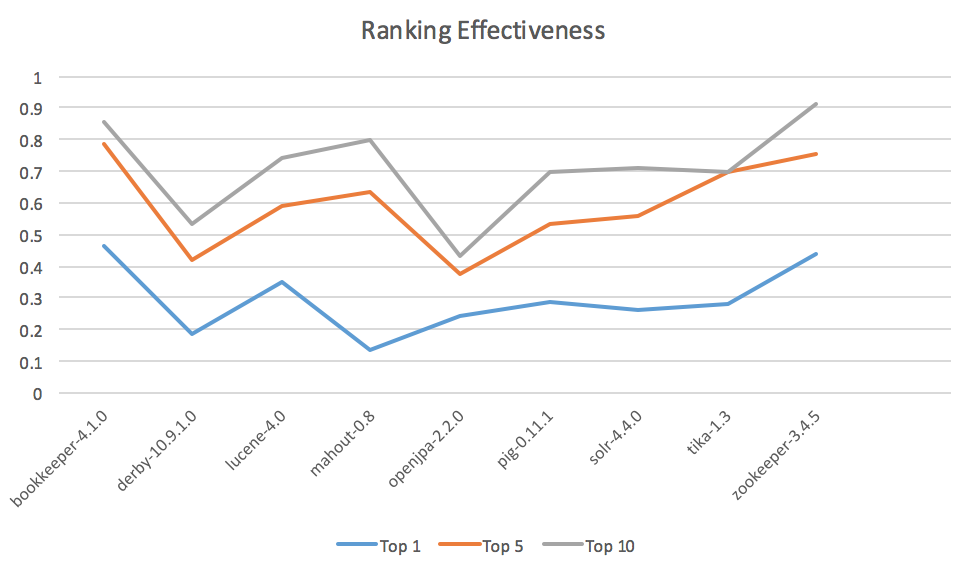
\includegraphics[scale=.5]{ranking}
\subsection{Experimental Data}

\begin{figure}
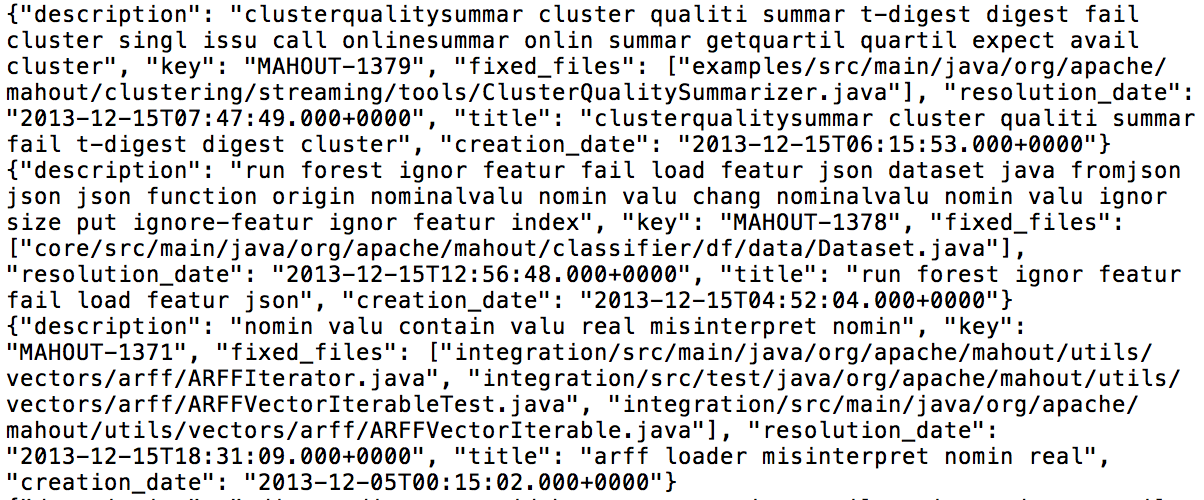
\includegraphics[scale=.38]{json}
	\caption{Processed bug reports}
\end{figure}




\begin{figure}
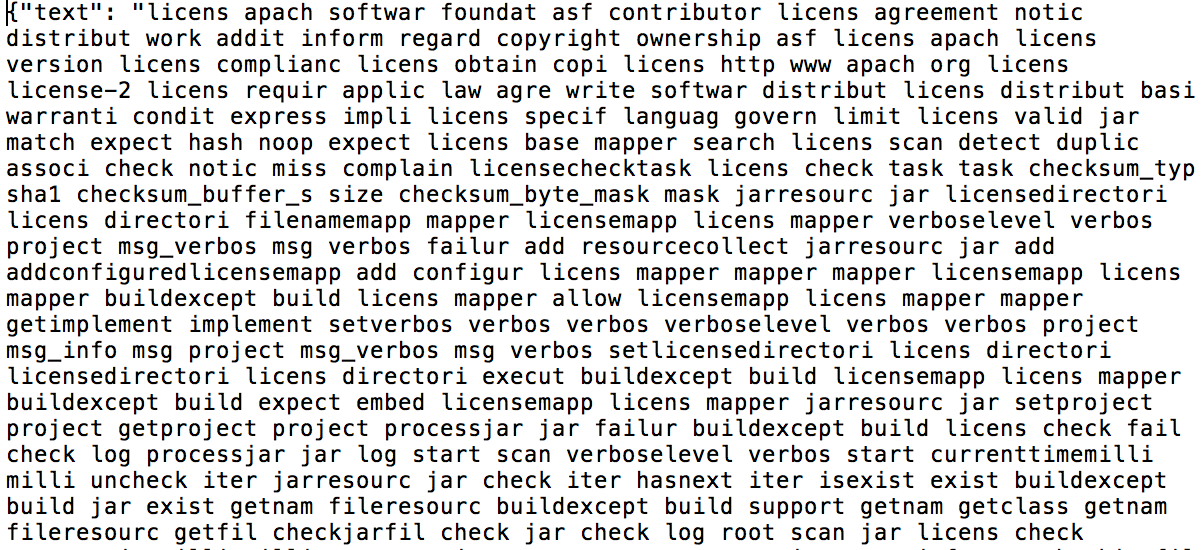
\includegraphics[scale=.38]{jsonSource}
	\caption{Processed source code files }
\end{figure}
 
\subsection{Evaluation and Experiments}

\subsection{Comparison Against Lucene}
\subsection{Limitations}
\subsection{Performance}

\section{Related Work}





\section{Challenges}
Several challenges arose during the development of the project. The Implementation of the specific scoring functions in order to obtain the ranked files with the possible bug location required a lot of investigation. There was a need to implement custom classes in Lucene in order to perform the search queries, assign weight to source code files and rank such files with a scorer class. 
Other challenges include the manual extraction of bugs reports from issue tracking system. While this process could be automated to read the content of issue tracking websites, we found that there is not an standardized form of submitting and reporting bugs. While some programs had very well organized reports with the patches attached stating the specific location of the bug, other contained no fix for the bug or repeated bug reports with the solution stated on the comments.

\section{Future Work}
There is a need to improve several aspects of the project in order to improve its effectiveness. One aspect that is important to mention is increasing the granularity of the tool. We are currently implementing granularity at the source code level. By refining the granularity to a method level, our framework will be able to present programmers a smaller piece of code and hence ease the effort when trying to locate and fix a bug. Another aspect that could be improved is the automation of bug extraction from issue tracking systems. This could potencially enhance the process for fixing bugs by presenting users with possible locations at the method level as soon as users enter bug reports. 

\section{Conclusion}
With our implementation, we aim at developing a tool for bug localization at the file level that takes bug reports
as input. This implementation uses a similar technique used in already known tools such as BugLocator. We will
also test the effectiveness of our tool on a gold set constructed from open source projects. With these results,
a comprehensive analysis of the strengths and weaknesses of the approach will be carried out, which will allow
us to propose candidates for future work.

\bibliographystyle{abbrv}
\bibliography{project}
\balancecolumns


\begin{table}[t]
    \begin{tabular}{|l|l|l|l|l|l|l|l|l|l|}
    \hline
        System           &     Alpha &     Top 1   &     Top 5   &     Top 10  &     MRR     &     MAP     &     Avg.   Precision &     Avg.   Recall & Queries \\ \hline
        bookkeeper-4.1.0 &     0.3   &     46.39\% &     78.35\% &     85.57\% &     58.49\% &     44.77\% &     44.77\%             &     97.71\%          &     97            \\ \hline
        derby-10.9.1.0   &     0.3   &     18.52\% &     41.98\% &     53.09\% &     29.75\% &     24.10\% &     24.10\%             &     99.45\%          &     162           \\ \hline
        lucene-4.0       &     0.3   &     34.85\% &     59.09\% &     74.24\% &     47.63\% &     37.01\% &     37.01\%             &     99.49\%          &     66            \\ \hline
        mahout-0.8       &     0.3   &     13.33\% &     63.33\% &     80.00\% &     33.81\% &     26.05\% &     26.05\%             &     98.19\%          &     30            \\ \hline
        openjpa-2.2.0    &     0.3   &     24.32\% &     37.84\% &     43.24\% &     31.11\% &     24.48\% &     24.48\%             &     100.00\%         & 37                \\ \hline
        pig-0.11.1       &     0.3   &     28.57\% &     53.57\% &     69.64\% &     43.18\% &     33.02\% &     33.02\%             &     100.00\%         &     56            \\ \hline
        solr-4.4.0       &     0.3   &     26.00\% &     56.00\% &     71.00\% &     40.40\% &     31.46\% &     31.46\%             &     98.20\%          &     100           \\ \hline
        tika-1.3         &     0.3   &     27.91\% &     69.77\% &     69.77\% &     43.61\% &     38.00\% &     38.00\%             &     97.67\%          &     43            \\ \hline
        zookeeper-3.4.5  &     0.3   &     43.90\% &     75.61\% &     91.46\% &     57.07\% &     44.62\% &     44.62\%             &     97.45\%          &     82            \\ \hline
    \end{tabular}
	\caption {IR Performance}
\end{table}


\end{document}
